\section{Radiative Transfer Results}
To validate the developed RTM, results from disk-averaged computations were compared to various disk-averaged brightness measurements taken of Venus. Table \ref{tab:rtm-results} shows results for measurements of the microwave and millimeter-wave disk-averaged brightness temperatures of Venus. For comparison purposes the table also shows the computed disk-averaged brightness temperatures ($T_D$) for Venus using the developed RTM. 

For the lower frequencies our computed $T_D$ is much higher then the measured values. This is likely due to the relatively simple model used for surface emissivity. The larger values computed at higher frequencies are likely due to the value assumed for $SO_{2_{surf}}$, (75 ppm) and could be adjusted by changing that value.%This is due to the understatement of the H$_2$SO$_4$ abundance profile. Since H$_2$SO$_4$'s profile varies widely by latitude and longitude using a different profile will make this difference much smaller. 

Figure \ref{fig:weight} shows the weighting function of various frequencies. Changing the SO$_2$ and H$_2$SO$_4$ abundance profiles will results in a change in the weighting functions as well as the disk-averaged temperature.
\begin{table}[h]
 \centering 
\caption{Measured Disk-Averaged Brightness Temperatures of Venus for Various Frequencies as compared to the reults from the new Radiative Transfer Model}
\begin{tabular}{||c|c|c|c|c||}
\hline
Frequency & Wavelength & Measured $T_D$ & Computed $T_D$ & Reference\\
(GHz) & (cm) &(K)&(K)& of Measurements\\
\hline
1.385 	& 21.66	 	&$612.8 \pm 12.3$	&642.6  &Butler et al., 2001 			\cite{Butler-2001}\\
1.42 	& 21.12 	&$617 	\pm 25$		&642.7  &Berge et al., 1972 			\cite{Berge-1972}\\
1.5 	& 20.00 	&$636 	\pm 28$		&643.1  &Pettengill et al., 1988 		\cite{Pettengill-1988}\\
2.91 	& 10.31 	&$620 	\pm 30$		&651.4  &Vetukhnovkaya et al., 1969 	\cite{Vetukhnovkaya-1969}\\
4.86 	& 6.41	 	&$679.9 \pm 13.6$	&654.1  &Butler et al., 2001 			\cite{Butler-2001}\\
5.0 	& 6.0 		&$652 	\pm 30$		&653.7  &Berge et al., 1972 			\cite{Berge-1972}\\
8.42 	& 3.56	 	&$652 	\pm 15$		&621.3  &Steffes et al., 1990 			\cite{Steffes-1990}\\
8.44 	& 3.55	 	&$657.5 \pm 13.2$	&621.0  &Butler et al., 2001 			\cite{Butler-2001}\\
9.62 	& 3.12	 	&$608 	\pm 35$		&605.4  &Berge et al., 1972 			\cite{Berge-1972}\\
11.11 	& 2.70	 	&$612 	\pm 37$		&585.9  &McCullough et al., 1972 		\cite{McCullough-1972}\\
13.3	& 2.26	 	&$561 	\pm 19$		&559.3  &Steffes et al., 1990			\cite{Steffes-1990}\\
14.94 	& 2.00	 	&$565.8 \pm 17$		&542.1  &Suleiman et al., 1997 			\cite{Suleiman-thesis}\\
14.94 	& 2.00	 	&$565.9 \pm 17$		&542.1  &Butler et al., 2001 			\cite{Butler-2001}\\
18.46 	& 1.63	 	&$520 	\pm 17$		&511.2  &Steffes et al., 1990			\cite{Steffes-1990}\\
22.25 	& 1.35	 	&$507 	\pm 22$		&485.0  &Steffes et al., 1990			\cite{Steffes-1990}\\
22.46 	& 1.34	 	&$505.2 \pm 25.3$	&483.7  &Butler et al., 2001 			\cite{Butler-2001}\\
22.46 	& 1.34	 	&$499.1 \pm 25$		&483.7  &Suleiman et al., 1997 			\cite{Suleiman-thesis}\\
37.50 	& 0.80	 	&$440 	\pm 35$		&421.6  &Vetukhnovkaya et al., 1969 	\cite{Vetukhnovkaya-1969}\\
86.1 	& 0.35	 	&$357.5	\pm 13.1$	&345.7  &Ulich et al., 1980 			\cite{Ulich-1980}\\
\hline
\end{tabular}
\label{tab:rtm-results}
\end{table}

\begin{figure}[p]
    \centering
	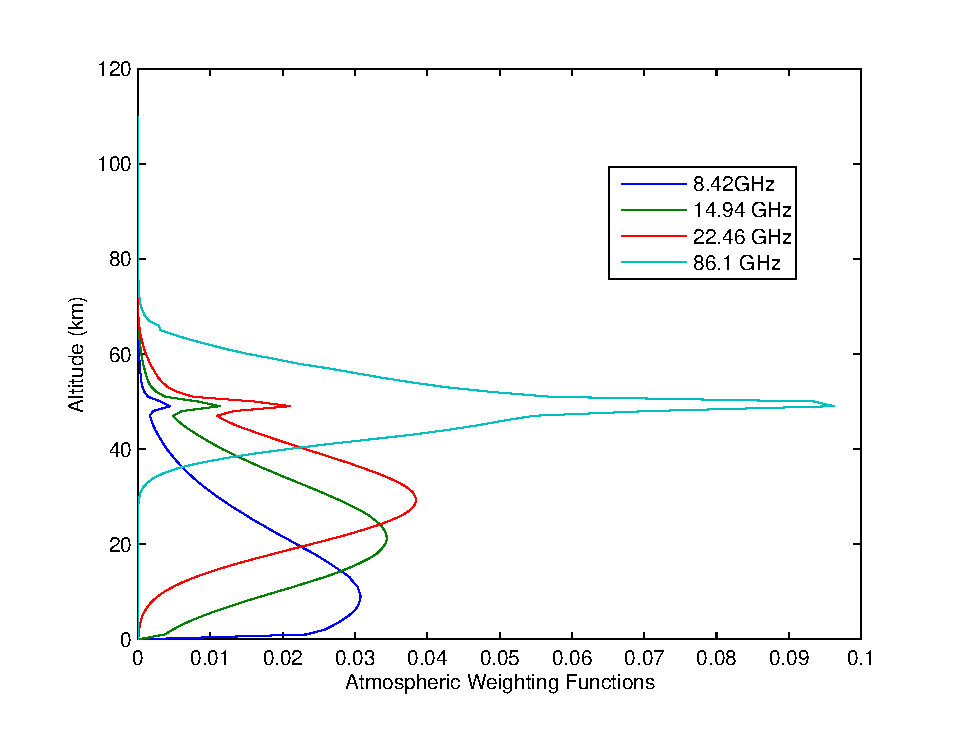
\includegraphics[width=0.7\textwidth]{./rtm/plots/weight.eps}
	\caption{Disk-averaged weighting function of the Venus atmosphere at frequencies of 8.42, 14.94, 22.46, and 86.1 GHz. }
		\label{fig:weight}
\end{figure}